\documentclass{sig-alternate-ipsn13}

\begin{document}

\title{Touchless Countdown Clock: No Soiled Interface Anymore }
%
% You need the command \numberofauthors to handle the 'placement
% and alignment' of the authors beneath the title.
%
% For aesthetic reasons, we recommend 'three authors at a time'
% i.e. three 'name/affiliation blocks' be placed beneath the title.
%
% NOTE: You are NOT restricted in how many 'rows' of
% "name/affiliations" may appear. We just ask that you restrict
% the number of 'columns' to three.
%
% Because of the available 'opening page real-estate'
% we ask you to refrain from putting more than six authors
% (two rows with three columns) beneath the article title.
% More than six makes the first-page appear very cluttered indeed.
%
% Use the \alignauthor commands to handle the names
% and affiliations for an 'aesthetic maximum' of six authors.
% Add names, affiliations, addresses for
% the seventh etc. author(s) as the argument for the
% \additionalauthors command.
% These 'additional authors' will be output/set for you
% without further effort on your part as the last section in
% the body of your article BEFORE References or any Appendices.

\numberofauthors{1} %  in this sample file, there are a *total*
% of EIGHT authors. SIX appear on the 'first-page' (for formatting
% reasons) and the remaining two appear in the \additionalauthors section.
%
\author{
% You can go ahead and credit any number of authors here,
% e.g. one 'row of three' or two rows (consisting of one row of three
% and a second row of one, two or three).
%
% The command \alignauthor (no curly braces needed) should
% precede each author name, affiliation/snail-mail address and
% e-mail address. Additionally, tag each line of
% affiliation/address with \affaddr, and tag the
% e-mail address with \email.
%
% 1st. author
\alignauthor
Chun-Yen Hsu\\
       % \titlenote{Dr.~Trovato insisted his name be first.}\\
       \affaddr{Carnegie Mellon University}\\
       \affaddr{94035 Mountain View}\\
       \affaddr{California, USA}\\
       \email{chunyenh@andrew.cmu.edu}
% Ben Trovato\titlenote{Dr.~Trovato insisted his name be first.}\\
%        \affaddr{Institute for Clarity in Documentation}\\
%        \affaddr{1932 Wallamaloo Lane}\\
%        \affaddr{Wallamaloo, New Zealand}\\
%        \email{trovato@corporation.com}
% % 2nd. author
% \alignauthor
% G.K.M. Tobin\titlenote{The secretary disavows
% any knowledge of this author's actions.}\\
%        \affaddr{Institute for Clarity in Documentation}\\
%        \affaddr{P.O. Box 1212}\\
%        \affaddr{Dublin, Ohio 43017-6221}\\
%        \email{webmaster@marysville-ohio.com}
% % 3rd. author
% \alignauthor Lars Th{\o}rv{\"a}ld\titlenote{This author is the
% one who did all the really hard work.}\\
%        \affaddr{The Th{\o}rv{\"a}ld Group}\\
%        \affaddr{1 Th{\o}rv{\"a}ld Circle}\\
%        \affaddr{Hekla, Iceland}\\
%        \email{larst@affiliation.org}
% \and  % use '\and' if you need 'another row' of author names
% % 4th. author
% \alignauthor Lawrence P. Leipuner\\
%        \affaddr{Brookhaven Laboratories}\\
%        \affaddr{Brookhaven National Lab}\\
%        \affaddr{P.O. Box 5000}\\
%        \email{lleipuner@researchlabs.org}
% % 5th. author
% \alignauthor Sean Fogarty\\
%        \affaddr{NASA Ames Research Center}\\
%        \affaddr{Moffett Field}\\
%        \affaddr{California 94035}\\
%        \email{fogartys@amesres.org}
% % 6th. author
% \alignauthor Charles Palmer\\
%        \affaddr{Palmer Research Laboratories}\\
%        \affaddr{8600 Datapoint Drive}\\
%        \affaddr{San Antonio, Texas 78229}\\
       % \email{cpalmer@prl.com}
}
% There's nothing stopping you putting the seventh, eighth, etc.
% author on the opening page (as the 'third row') but we ask,
% for aesthetic reasons that you place these 'additional authors'
% in the \additional authors block, viz.
\additionalauthors{Additional authors: John Smith (The Th{\o}rv{\"a}ld Group,
email: {\texttt{jsmith@affiliation.org}}) and Julius P.~Kumquat
(The Kumquat Consortium, email: {\texttt{jpkumquat@consortium.net}}).}
\date{30 July 1999}
% Just remember to make sure that the TOTAL number of authors
% is the number that will appear on the first page PLUS the
% number that will appear in the \additionalauthors section.

\maketitle
\begin{abstract}

We present an touchless countdown clock that provides an innovative interactive way for users to set clock without actually touching the display.
\end{abstract}

\section{Introduction}

Traditional countdown clock provides the time choice function with physical button for users to select how long times we want to count. After the time is decided, we can press the "start" button then the clock start counting down the time. However, under some restrictive circumstances, such as performing surgeon which requires undust hand and is prohibited to touch unnecessary things, or cooking with greasy hands but still need to use countdown clock for keeping time, buttons would not be a good way to let users interact with the clock. 
% Besides, grease or heavy metal ingredients on our hand would let us feel anguished to touch expensive clock devices.

We present touchless countdown clock(Figure \ref{fig:demo1}), which utilize light sensor with high-sensitivity photodiode to implement touchless function as an innovative human interface application with no physical contact necessary.
Light sensor would detect whether users' hand appears in front of the device. Whenever it finds the hand shake, it will add one minute to the countdown clock and start counting the time automatically. This implementation can definitely solve the problem that user does not require to touch the clock anymore. Touchless function not only simplifies the manipulation interface but it release the user restriction under certain environment limitation.
 

% innovative touchless human interface applications
% The high-sensitivity infrared photodiode provides a single-pulse infrared proximity measurement, offering customers an opportunity to implement a proximity and ambient light sensor with very low power levels.


% \begin{figure}
% \centering
% 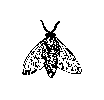
\epsfig{file=fly.eps}
% \caption{A sample black and white graphic (.eps format).}
% \label{fig:example}
% \end{figure}

\begin{figure}
  \centering
  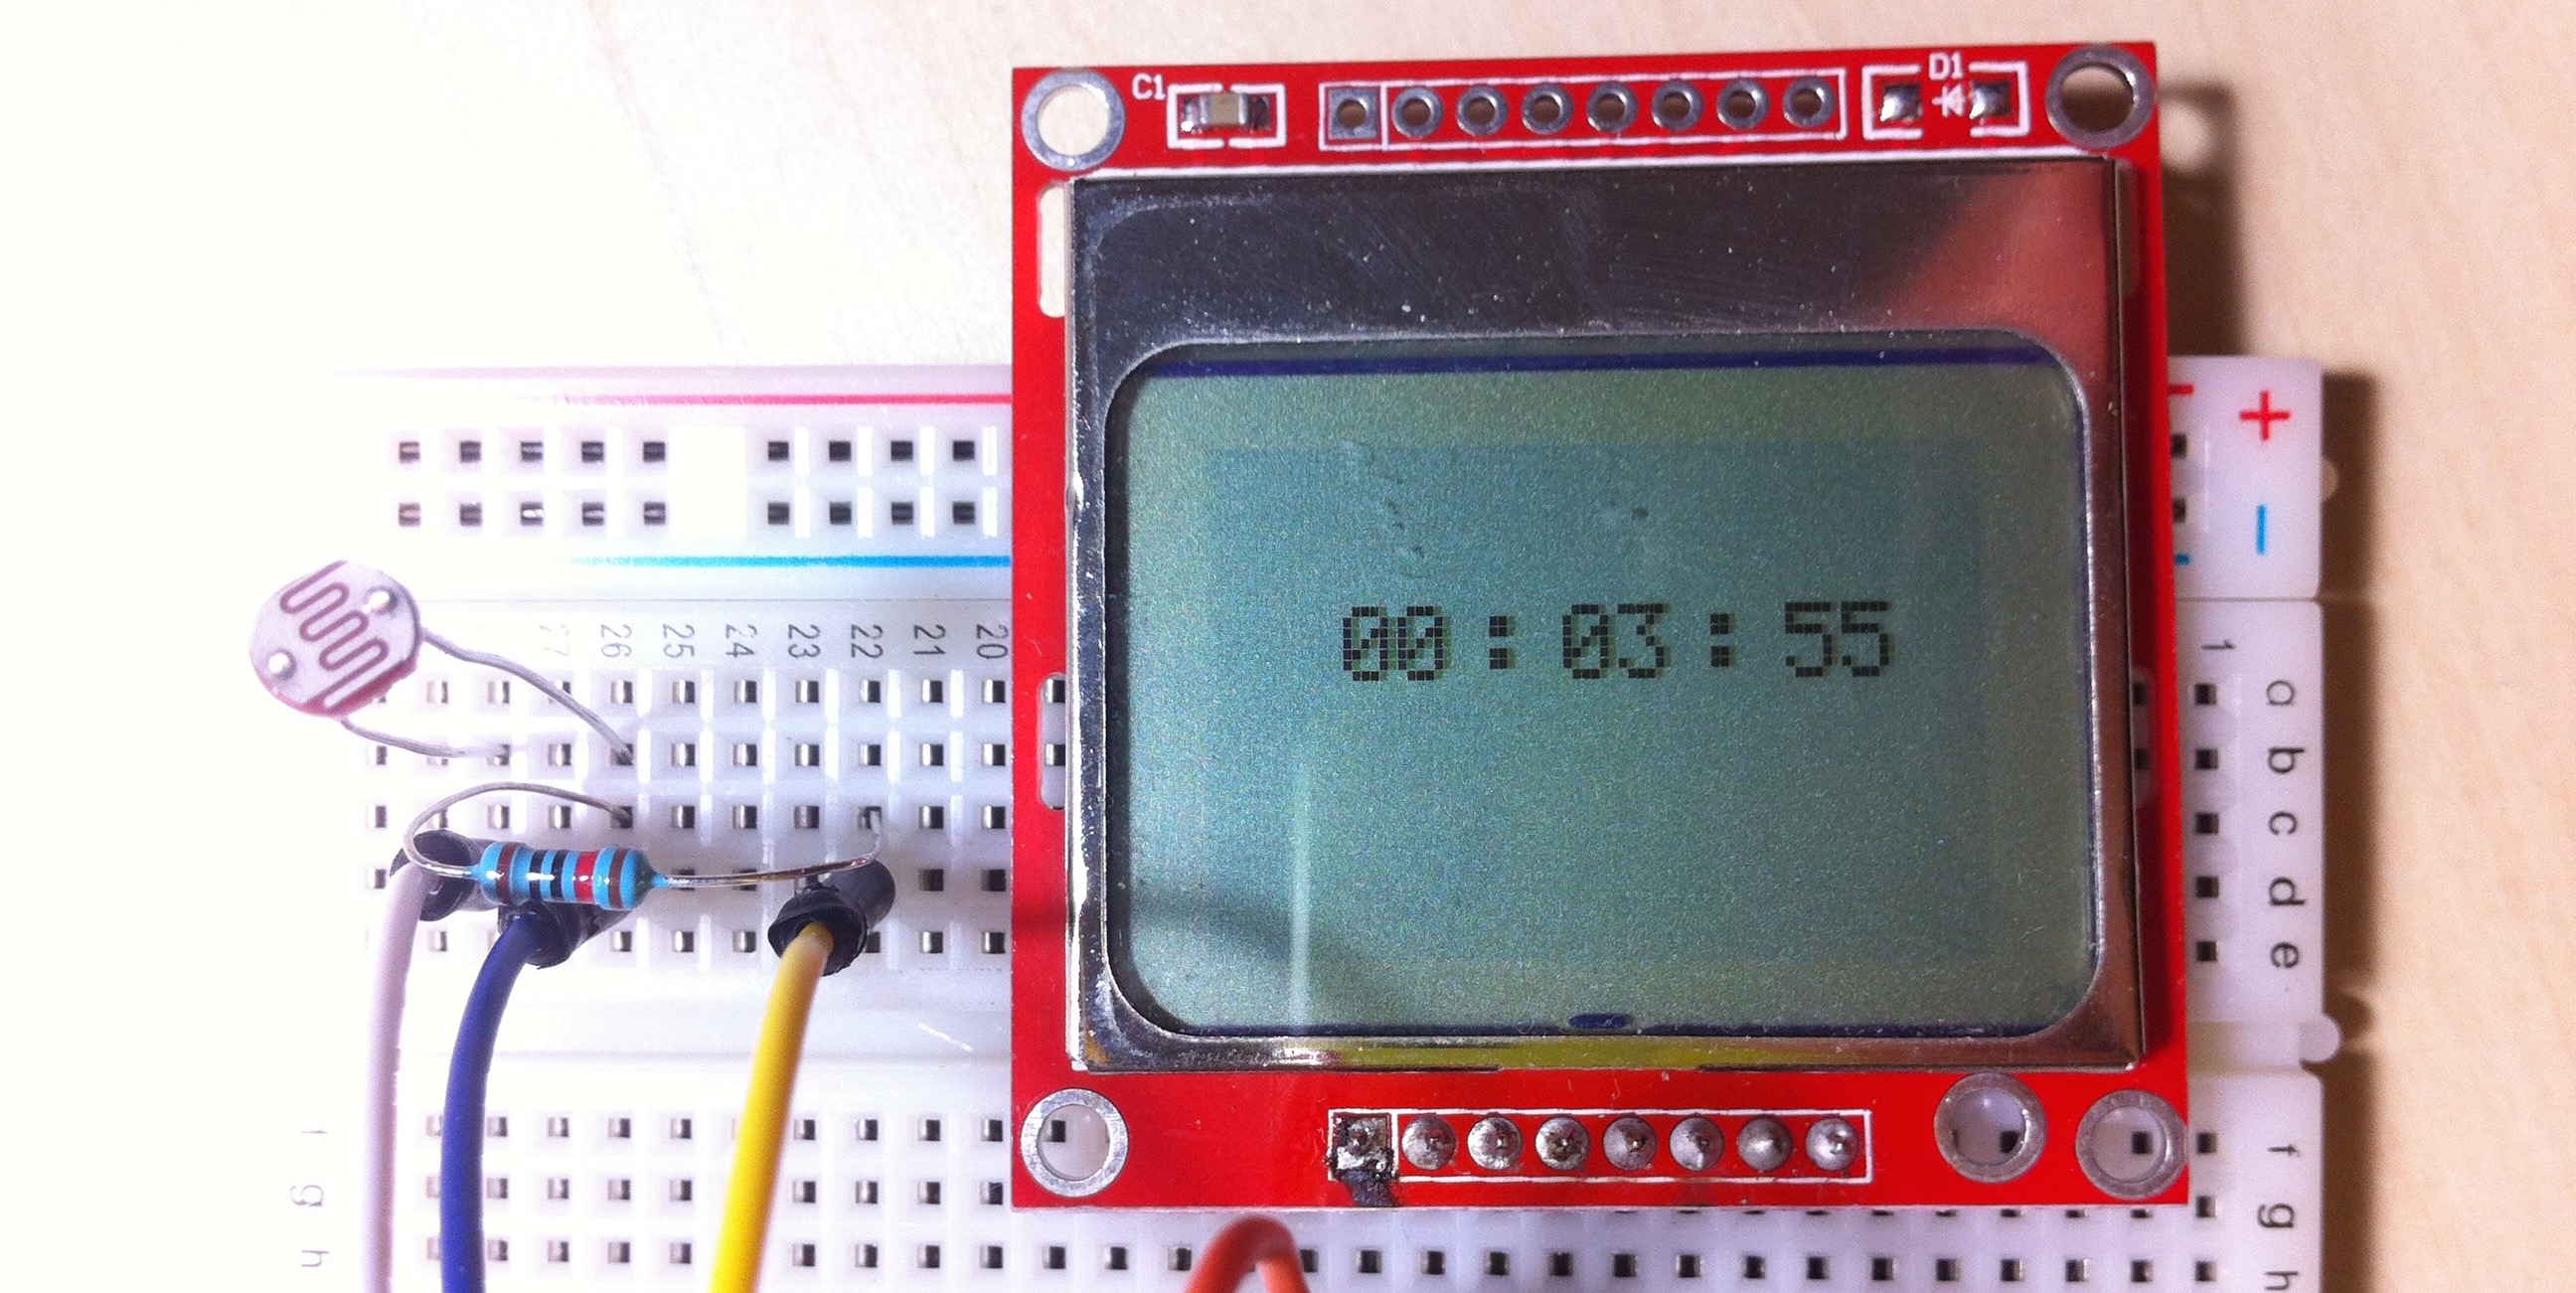
\includegraphics[width=0.9\linewidth]{Figures/demo1.jpg}
  \caption{Touchless Countdown Clock with light sensor at the left of the figure}
  \label{fig:demo1}
\end{figure}

\section{Related Work}
We found a research work Touchless Circular menus\cite{cite1}, which explores touchless interaction in diverse usage contexts, such as interacting with public displays where mouse and keyboards are inconvenient. This idea is also ideal to face our problem that can be used as activating kitchen devices without touching them with dirty hands.

%%Citation Abstract
% Researchers are exploring touchless interactions in diverse usage contexts. These include interacting with public displays, where mouse and keyboards are inconvenient, activating kitchen devices without touching them with dirty hands, or supporting surgeons in browsing medical images in a sterile operating room. 
% Unlike traditional visual interfaces, however, touchless systems still lack a standardized user interface language for basic command selection (e.g., menus). Prior research proposed touchless menus that require users to comply strictly with system-defined postures (e.g., grab, finger-count, pinch). These approaches are problematic because they are analogous to command-line interfaces: users need to remember an interaction vocabulary and input a pre-defined symbol (via gesture or command). To overcome this problem, we introduce and evaluate Touchless Circular Menus (TCM)---a touchless menu system optimized for large displays, which enables users to make simple directional movements for selecting commands. TCM utilize our abilities to make mid-air directional strokes, relieve users from learning posture-based commands, and shift the interaction complexity from users' input to the visual interface. In a controlled study (N=15), when compared with contextual linear menus using grab gestures, participants using TCM were more than two times faster in selecting commands and perceived lower workload. However, users made more command-selection errors with TCM than with linear menus. The menu's triggering location on the visual interface significantly affected the effectiveness and efficiency of TCM. Our contribution informs the design of intuitive UIs for touchless interactions with large displays.


\section{Conclusions}
Conclusion goes here.

%ACKNOWLEDGMENTS are optional
% \section*{Acknowledgments}
% Acknowledgement goes here.

%
% The following two commands are all you need in the
% initial runs of your .tex file to
% produce the bibliography for the citations in your paper.
\bibliographystyle{abbrv}
\bibliography{sigproc}  % sigproc.bib is the name of the Bibliography in this case
% You must have a proper ".bib" file
%  and remember to run:
% latex bibtex latex latex
% to resolve all references
%
% ACM needs 'a single self-contained file'!
%
%APPENDICES are optional
%\balancecolumns
% \appendix
%Appendix A

% Appendix goes here.

% That's all folks!
\end{document}
